% AuctionNet の解説（教授向けの前提資料）。.claude/commands/make_document.md の手順でコンパイルする。
% 図は論文（Su et al., NeurIPS 2024）の Figure 1, 10 を切り出したもの。
\documentclass[twocolumn, a4paper, 10pt]{ujarticle}
\usepackage{doc_format}
\usepackage[font=small]{caption}
\setlist{nosep,leftmargin=1.4em}

\begin{document}
\doctitle{AuctionNet：大規模広告オークションにおける自動入札のベンチマーク\\と，本研究の位置づけ}
\docinfo{2026年10月12日　ミーティング資料}
\maketitle

% ============================================================
\section{はじめに}
% ============================================================

研究テーマを変更した。前のテーマは，共通のベンチマークがなく，手法の比較や検証がやりづらかった。
一方で，前の研究を通じて，広告・マーケティングサイエンスという応用領域に興味を持った。
この領域を軸に研究内容を再検討する中で，ベンチマーク \textbf{AuctionNet}\,\cite{su2024} を見つけた。

AuctionNet は，広告オークションで広告主に代わって自動で入札する\textbf{自動入札エージェント}のアルゴリズムを，共通の条件で評価するためのベンチマークである。
広告オークションのシミュレーション環境，それを使って生成した大規模データセット，代表的な手法の性能評価の3つからなる。
このベンチマークを基盤として，NeurIPS 2024 のコンペティション「Auto-Bidding in Large-Scale Auctions」が開催され，
世界中から 1,500 を超えるチームが，入札アルゴリズムの精度を競った。

本研究では，この AuctionNet を使って，次のいずれか（または両方）を行い，その結果を根拠に，自分なりの新しい入札手法を提案したい。
(a) 既存手法の問題点を解明する。
(b) 最も成績の良かった既存手法（論文のベースライン評価では Online LP）が，なぜうまくいくのかを，理論的・実験的に詰める。

本稿では，今回取り組む AuctionNet のベンチマーク問題を詳しく説明する。
2章で論文の内容を要約し，3章で本研究の目的を述べる。
広告の分野に馴染みがなくても読めるよう，用語は初出の箇所で説明する（表\ref{tab:terms}）。

\begin{table}[H]
\centering
\caption{本稿で使う広告用語}
\label{tab:terms}
\footnotesize
\begin{tabularx}{\linewidth}{@{}lX@{}}
\toprule
広告機会（インプレッション機会） & ユーザーがページを開くたびに生じる，広告を表示する権利。1回ごとにオークションにかけられる \\
コンバージョン（CV） & 広告を見たユーザーが購入などに至ること。広告主が最終的に欲しい成果 \\
価値 & ある広告機会でコンバージョンが起きる確率の予測値（pCTR $\times$ pCVR）。環境が計算して入札前に渡す \\
予算・CPA 制約 & 予算：期間内に使える費用の上限。CPA：コンバージョン1件あたりの費用の上限 \\
GSP オークション & 一般化セカンドプライス。落札者は，自分の入札額ではなく，次点の入札額付近を支払う \\
\bottomrule
\end{tabularx}
\end{table}

% ============================================================
\section{AuctionNet の解説（論文の要約）}
% ============================================================

\subsection{背景と課題}

オンライン広告の多くは，広告を表示する権利をリアルタイムのオークションで売買する\textbf{リアルタイム入札（RTB）}で取引される（2023年の市場規模は 6,000 億ドル超）。
ユーザーがページを開く度に広告機会が発生し，広告主は，予算や CPA などの制約の下で成果（コンバージョン数など）を最大化したい。
機会は膨大で人手では入札できないため，広告主ごとの\textbf{自動入札エージェント}が，連続して到着する機会に代わりに入札する（図\ref{fig:overview}）。
各エージェントは他の広告主の戦略を知らないまま競争するので，これは多数のエージェントが競う大規模なゲームにおける意思決定である。

研究上の課題は，現実的な環境に研究者がアクセスしにくいことである。
既存の環境には，AuctionGym（予算の時間変化を扱わない）や AdCraft（競合の入札を分布からのサンプリングで表すため，競争の動的な性質を捉えきれない）があるが，実環境との隔たりが大きい。
そこで AuctionNet は，実際のオンライン広告プラットフォームに由来する環境・データセット・ベースライン評価を一式で提供する。

\begin{figure*}[t]
\centering
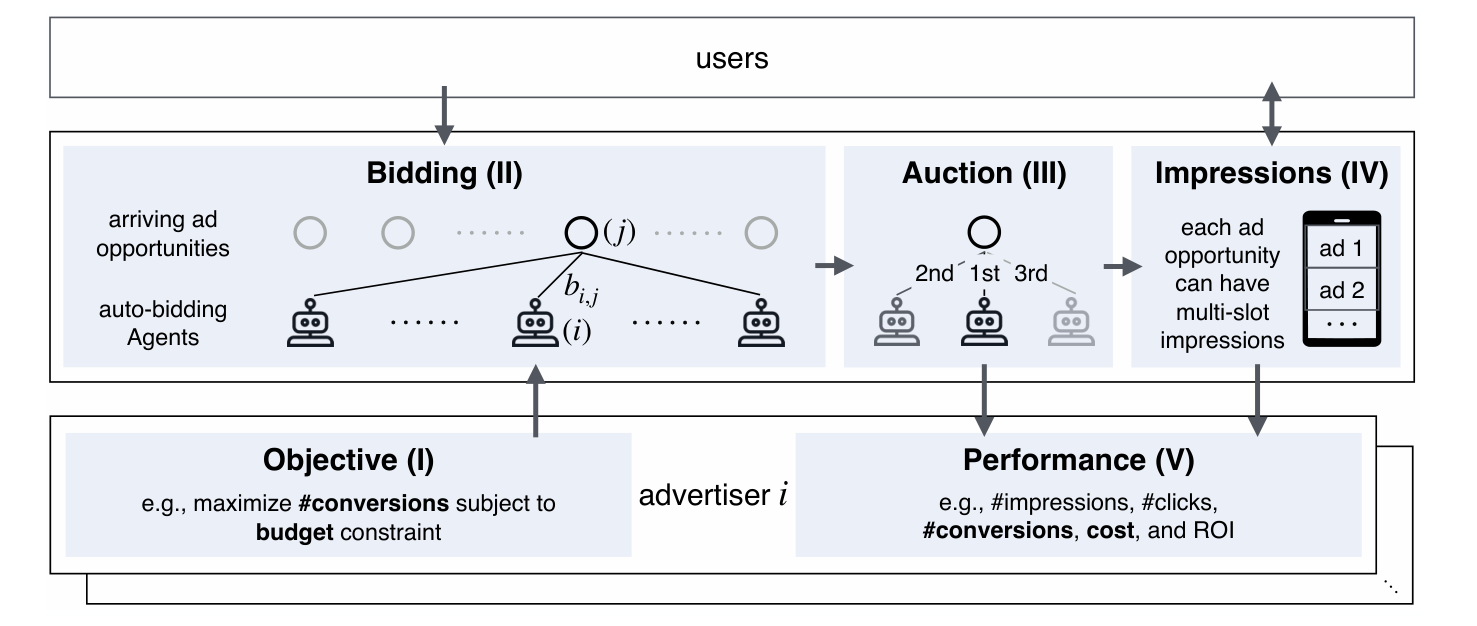
\includegraphics[width=0.8\textwidth]{figs/fig1_overview.png}
\caption{大規模オンライン広告プラットフォームの概要（論文 Figure 1）。広告主 $i$ の目的（I）に対し，エージェントが広告機会ごとに入札し（II），オークション（III）で競争して，インプレッション（IV）と成果（V）を得る。}
\label{fig:overview}
\end{figure*}

\subsection{対象とする問題：自動入札}

問題は，部分観測確率ゲーム（POSG）として定式化される。エージェント $i$ が観測するのは状態の一部で，たとえば他のエージェントの予算は知らない場合がある。
1期間（エピソード）は $T$ 個の意思決定ステップに分割され，各ステップで，エージェントは\textbf{入札係数 $\alpha_i$ を1つだけ}決める。
「最適な入札額は広告機会の価値に比例する」という既知の結果 \cite{balseiro2015} に従い，広告機会 $j$ への入札額は $b_{ij}=\alpha_i v_{ij}$（$v_{ij}$ は価値）とする。
落札した機会 $x_{ij}=1$ からだけ，価値 $v_{ij}$ の報酬を得て，コスト $c_{ij}$ を支払う。
典型的な目的は，予算制約付きの獲得価値の最大化である。
\begin{equation}
\max_{\{\alpha_i^t\}}\ \sum_{t=1}^{T}\langle x_i^t, v_i^t\rangle
\quad\text{s.t.}\quad \sum_{t=1}^{T}\langle x_i^t, c_i^t\rangle \le \omega_i
\tag{1}
\end{equation}
ここで $\omega_i$ は予算である。より現実的な設定として，CPA 制約を加えた目標 CPA タスクがあり，制約を超えると成績にペナルティが掛かる（論文の付録 E）。
決定変数が各ステップの係数 $\alpha$ だけであり，どの手法も，この $\alpha$ の決め方が違うだけである。

\subsection{広告オークション環境}

1期間を 48 ステップに分け，ステップ内の広告機会は並列に処理する。環境は，次の3つのモジュールの相互作用で，実際の広告オークションを再現する。
\begin{itemize}
\item \textbf{広告機会生成モジュール}：機微な実データの漏洩を避けつつ実データに近い機会を作るため，深層生成モデルを使う。広告機会の特徴量は\textbf{潜在拡散モデル}で生成し，価値は Multi-head Attention による予測モデルで，広告主のカテゴリと時刻を取り込んで付与する。時間帯による機会の量の変動も再現する。
\item \textbf{入札モジュール}：広告主ごとに異なる目的を持つ多数の自動入札エージェントを置く。競合として，PID，Online LP，IQL，BC，Decision Transformer（DT）が実装されている。研究者は一部のエージェントだけを制御し，他は制御できない。
\item \textbf{オークションモジュール}：GSP を基本とし，独自のルールも設計できる。1つの機会が複数のスロットを持ち，露出率の高いスロットほど価値が高い。露出率が価値とコストの両方に掛かるため，最適な入札は複雑になる。
\end{itemize}
環境は Python で実装され，API は OpenAI Gym に似る。

\subsection{事前生成データセット}

この環境で，多数のエージェントを競争させて生成したデータセットが公開されている。
1,000 万件の広告機会（21 エピソード，各 50 万件超を 48 ステップに分割），各機会の入札上位 48 エージェント，5 億件超のレコード，合計 80\,GB で，
予測価値，入札，オークション結果，インプレッション結果が含まれる。環境のモデル化や，入札エージェントの学習に使える。
生成モデルの妥当性は，実データ 10 万件との比較で確認されている（PCA で似たクラスタ構造，属性・消費行動の分布，ロングテール，カテゴリと時刻に応じた価値の変動）。
データの分析からは，カテゴリごとに価値の時間変動が違うこと，カテゴリ間に相関（類似の機会を巡る競合）があることが示され，入札のタイミングと競合の考慮が重要だと示唆される。
一方，著者は，生成データと実データには一部に偏り（例：稀なカテゴリ）が残ることを限界として挙げている。

\subsection{ベースラインアルゴリズムの性能評価}

PID，Online LP，IQL，Behavior Cloning（BC），DT，および基準となるヒューリスティック Abid（固定の入札率）を，予算制約のみの\textbf{基本タスク}と\textbf{目標 CPA タスク}で比較している（図\ref{fig:baseline}）。
いずれも元論文の手法をそのまま使い，自動入札向けの調整はしていない。性能は，Abid の平均報酬を 1.0 とした相対値で示される。
\begin{itemize}
\item \textbf{Online LP が最も良い}。著者は，Online LP が頑健で，自動入札への特別な適応を必要としないためだろうと述べている。
Online LP は，線形計画法を使い，各ステップで貪欲法によりナップサック問題を解く手法である（論文の記述）。公開コードの実装では，過去の記録から作った早見表（広告機会を費用対効果の高い順に並べた累積費用の表）を引き，残り予算に見合う係数を選ぶ形になっている。
\item IQL（オフライン強化学習）や BC（模倣学習）は Online LP ほどではないが，最適化した解法の提案で性能を大きく改善できることが観察されており，大きな改善の余地があるとされる。
\item 目標 CPA タスクで全手法の報酬が下がるのは，CPA 制約の超過に対するペナルティによる。
\end{itemize}

\begin{figure*}[t]
\centering
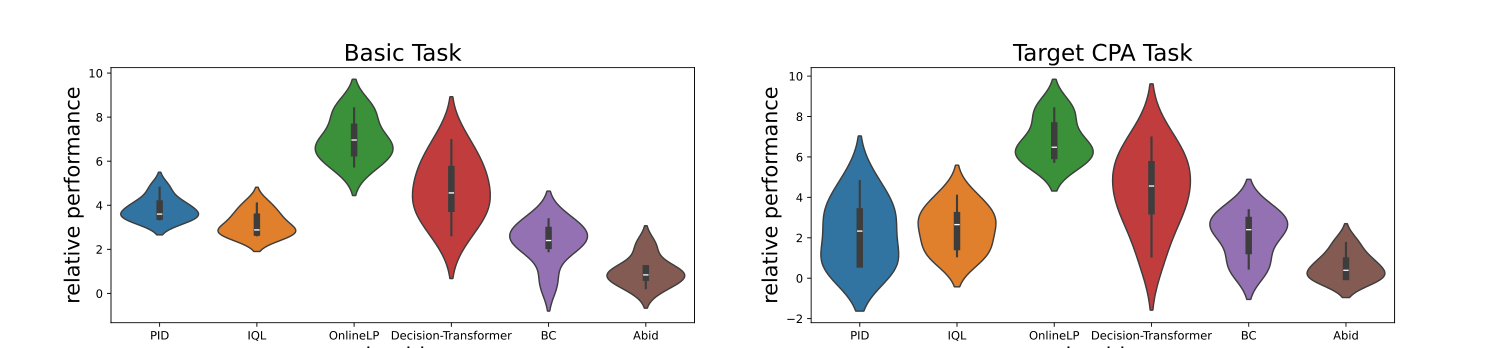
\includegraphics[width=0.8\textwidth]{figs/fig10_baselines.png}
\caption{ベースラインの実験結果（論文 Figure 10）。縦軸は Abid を基準とした相対性能。左：基本タスク，右：目標 CPA タスク。}
\label{fig:baseline}
\end{figure*}

\subsection{コンペティションでの利用}

AuctionNet は，NeurIPS 2024 のコンペティション「Auto-Bidding in Large-Scale Auctions」を支えた。
4 か月間，1,500 を超えるチームが参加し，環境は 1 万回近い評価を提供した。データセットとベースラインにより，参加者はすぐに課題に着手でき，多様な解法が生まれたと報告されている。

% ============================================================
\section{本研究の目的}
% ============================================================

AuctionNet は，実際の広告プラットフォームに由来する，大規模な入札ゲームの共通のベンチマークである。
そこでは，各ステップの入札係数 $\alpha$ を，先の見えない中でどう決めるかが問われる。
その中で最も成績が良かった既存手法（Online LP）についても，論文は「頑健だからだろう」と推測するにとどまり，なぜ良いのか，どこに限界があるのかは検証していない。
本研究の目的は，既存手法の問題点を解明するか，最良の手法がなぜうまくいくのかを理論的・実験的に詰め，その知見に基づいて，
自分なりの新しい入札手法を提案することである。

\begin{thebibliography}{9}\footnotesize
\bibitem{su2024} K.~Su, Y.~Huo, Z.~Zhang, S.~Dou, C.~Yu, J.~Xu, Z.~Lu, B.~Zheng. AuctionNet: A Novel Benchmark for Decision-Making in Large-Scale Games. NeurIPS 2024 Datasets and Benchmarks Track. arXiv:2412.10798.
\bibitem{balseiro2015} S.~R.~Balseiro, O.~Besbes, G.~Y.~Weintraub. Repeated auctions with budgets in ad exchanges: Approximations and design. Management Science 61(4):864--884, 2015.（論文の参考文献 [3]。「最適入札は価値に比例する」の出典として論文が挙げている。）
\end{thebibliography}

\end{document}
